\documentclass[10pt,a4paper]{article}

\usepackage{fullpage}
\usepackage{wrapfig}
\usepackage{lipsum}
\usepackage{hyperref}
\usepackage{cleveref}
\usepackage{tikz}
\usepackage{float}
\usepackage{comment}

\DeclareGraphicsExtensions{.pdf,.png,.jpg}

\begin{document}
\title{WebApp Group 34 Final Report}
\author{
  Han, Qiao\\
  \and
  Chabierski, Piotr\\
  \and
  Smith, Bradley\\
  \and
  Cingillioglu, Nuri\\
}

\maketitle

\section{Introduction}
Our project is a web based application that complements the process of creating and tracking of events and people who are attending the event. It also provides facilities to allow for participants to ask questions and find out information from the event organisers and for event organisers to control groups of people who are able to create events. 
\\
\\
\noindent This application contains two main entities:
\begin{description}
\item[Calendars] - these are entities that any user can create. User can subscribe to other peoples calendars where they can then be promoted to editors or admins. Depending on their role they will have different rights and available actions is described \textbf{put-link-here}.
\item[Events] - events are things that are created on the calendar they are available to join to anyone who is subscribed. They contain the following information, a title, a start date and time, an end end and time, a location, a max capacity (possibly unlimited) and a description.
\end{description}

\noindent We decided on creating this application due to a problem that one of our team members spotted during volunteering for the collage. This problem was with the way things were organised, which typically involves large quantities of emails to, send out the information, get responses back from interesting volunteers and either send out more telling people they are oversubscribed or asking for more people as they didn't get enough.
\\
\\
\noindent Our aims for this project were to improve our understanding of how to build a products by working with the purposed end users. We also aimed to gain an understanding of web development and database management along with a new range of technology in which most of us were novices. We have been working quite closely with the users to ensure that the features we have been implementing will appeal to them and can be integrated into their current work processes.
\\
\\
\noindent The basic requirements for our project were to make event organising easier (to do away with the huge amount of emails). We also gained quite a few requirements/possible extensions from conversing with the user.
\\
\\
\noindent There were (from meeting minutes):
\begin{itemize}
\setlength\itemsep{0.1em}
\item Allow event details to be edited after creation.
\item Allow admins to check who has signed up for an event they have created.
\item Allow for multiple admins on the same calendar to collaborate in setting up events. 
\item Make it so events can have prerequisites which users must identify they have read before they can sign up.
\item Allow admins to remove people from the events if they do not meet the prerequisites (or for any other reason).
\item Always start the calendar view on a Monday and highlight the current day.
\item Admin approval for events that were created by editors.
\item In-app live chat and offline messages for volunteers to ask questions and get answers.
\item Real time updates for new events and event subscriptions.
\item Make it easy to join and edit events from a mobile browser.  
\end{itemize}
\noindent We also got a lot more suggestions which we have either discarded due to coming up with a better alternative or put off in favour of more important features. Examples of these are email alerts of upcoming/important events, statistics on how much a user has volunteered (what events they have attended), report generation for events that have been created for each week, etc...

\section{Project Management}

\noindent The management of our project was realised with daily meetings to discuss progress and work out what we needed to work on each day. As we spend most of the time working in close proximity with each other it allowed us to communicate quickly on all matter which allowed us to easily minimize redundant work. We also used the user meetings (mentioned above) to help keep us on track.

\subsection{Group Structure}
\noindent We divided our group responsibilities based on our individual strengths. Han has done extensive development work on both server and client side applications in past internships and part time jobs and hence is the most suitable candidate for the role of group leader. The group leader is responsible for guiding the choices of technology together with ensuring a schedule for the timely completion of the project. In addition, he was also responsible for managing the team during evaluations of the project requirements and the suitability of different technology stacks in fulfilling our design goals.
\\
\\
\noindent
More specifically, our team members were initially in charge of working on following areas.

\begin{enumerate}
  \item Client-side presentation - Nuri
  \item Client-side interaction - Nuri / Han
  \item Server-side processing - Bradley / Piotr / Han
  \item Database set-up - Bradley / Piotr
\end{enumerate}

\noindent However as some things take longer then others, most of us ended up picking up things in other areas (mainly just patching stuff up). This was enabled by our close working conditions which meant that we could quickly ask whoever had implemented that area to explain the ideas or help fix bugs. We believe this was a good thing as it allowed us all to gain a general understanding of the bits we weren't assigned to, as well as a deep understanding of the bits we were. This helped us achieve our aims of getting a feel of the whole web application stack.   

\subsection{Implementation Choices}

Although we chose to use HTML, CSS, and Javascript for the frontend (for compatibility reasons), we have considered a wide variety of web development frameworks, ranging from full blown MVC frameworks such as AngularJS, MeteorJS, and Django templates, to minimalistic libraries such as jQuery, Backbone.js, and HTML5 Boilerplate. As the team was relatively new to web development, we decided to use frameworks that more closely represent the fundamental DOM layout to enhance our understanding. This means that HTML5 Boilerplate is a good choice because it consolidates the best practices of using modern web technologies without adding extra layers of abstraction. In addition, we have chosen to use the Bootstrap framework to enhance the visual presentation of our web app. Lastly, we decided to separate our data models from the views by fetching data asynchronously as JSON objects from our backend using RESTful APIs. Using RESTful APIs allows for easy integration with mobile clients while using JSON as the data format allows for transfer of rich data structures like nested objects and arrays.
\begin{comment}
  see also, closure, scala, dart, go, c++
\end{comment}
\\
\\
\noindent
We have picked a statically typed language, Java, as the implementation language for our backend. Although it may increase the amount of time needed to write our App, we believe the extra type safety combined with an active developer community makes it a good trade-off over other dynamically typed languages such as Python, node.js, and PHP. As most of us are familiar with Java, it is also easier to apply sound software design patterns that we have learnt over the course of our studies, such as singleton pattern or dependency injection/inversion. With the support of testing frameworks like JUnit and Mockito, we are able to provide good test coverage on our backend code base to ensure long term maintainability. This is especially important for our target market - enterprise web apps (see our App description). More generally, Java code is more habitable and allows for easier extension with its wide range of third party libraries. We also believe it will keep our options open going forward as it is very portable and platform independent.
\\
\\
%might want to expand on the use of Tomcat and PostgreSQL
\noindent
Lastly, we have decided to use Apache Tomcat as the web container and PostgreSQL as the database engine because they have been conveniently set up by CSG on lab machines.

\subsection{Design Processes}

As we tried to create as little coupling as possible between the front end and the back end, we used slightly different processes in designing and creating each one.  
\\
\\
\noindent For the front end we decided to first build a basic UI without any functionality. It allowed us to get an interface that was easy to understand, usable and fluid. It meant that half of the group could just focus on that for the start of the project. Next we added some basic functionality to see if it worked well and adjusted things if we thought they could be improved. From there we performed iterations of adding UI features $\rightarrow$ adding in the functionality $\rightarrow$ adjusting to achieve the desired look and feel of the components.
\\
\\
\noindent The back end design started with sketching out an outline the for API which achieved the basic functionality that we needed for the first set of features. Then we spent a fair amount of time re-factoring to improve readability , trying to include as many best practices as we could find and writing some tests to unsure that we hit all of the edge cases. Then we joined the design process for the front end in iterations of adding features $\rightarrow$ wiring them up to the front end $\rightarrow$ re-factoring if possible.     

\subsection{Backup Systems}

%Im not 100% sure what to write here
Gitlab came up as our method of choice for version control and backups (the choose was arbitrary). It has allowed us to ensure that all of our committed work is backed up and helps organise the project into different branches to its less likely for any work to be accidentally deleted. As far as database backups go we have not needed one so far as we have been regularly wiping it for table changes or because of inconsistent data use to testing. 

\section{Program and Implementation}

The basics of our application have already been covered in introduction and project management sections. Now we will go into details, starting with the overall system architecture and then going into the specific parts of the system.
\\
\\
\noindent Our system contains three independent parts, the front end (static web pages + javascript to provide calls to the API) the back end (the API, provides methods to access the main functionality of our system) and the database. The interactions are shown in the diagram below.

\begin{figure}[H]
\centerline{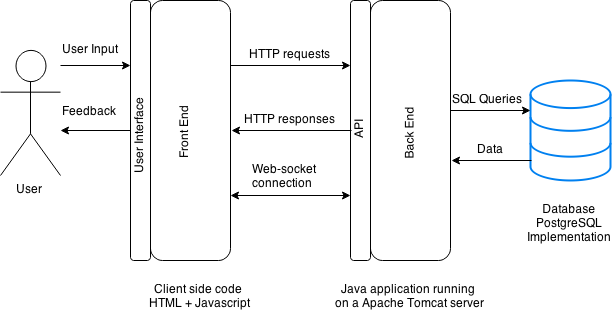
\includegraphics[scale=0.58,trim=0 0 100 0]{sysarch}}
\caption{System Architecture Diagram}
\end{figure}    


\section{Libraries}
Libraries that are used in the front-end:
\begin{description}
\item[jQuery] - We use version 2.1.4 which like any other version is licensed under the MIT license that permits any applicable usage. Although we could, we did not modify any sections of the library. https://jquery.com
\item[jQuery Datetime Picker] - We use this library to bind picking of date time input fields in the forms. Like jQuery the library is under the MIT license. http://xdsoft.net/jqplugins/datetimepicker/
\item[Bootstrap] - Bootstrap is also licensed under MIT. http://getbootstrap.com/
\item[Toastr Js] - MIT license. https://github.com/CodeSeven/toastr
\end{description}
It is important to note that all of the libraries the front-end uses are under the MIT license which means that we have the permission to reuse within proprietary software, for example we do not disclose the source code and charge for the usage, provided that all copies of the licensed software include a copy of the MIT License terms and the copyright notice. \\ \\
Libraries that are used in the back-end:
\begin{description}
\item[Google GSON] - The GSON library is used to serialize and deserialize Java objects into Json strings when they are sent to and recieved from the front-end. It is licensed under the Apache License 2.0. https://code.google.com/p/google-gson/
\item[PostgreSQL JDBC Driver] - The Java back-end is linked to the group database using the driver. Licensed under BSD license. https://jdbc.postgresql.org/
\end{description}
     
\newpage
\newpage
\section{To put somewhere later}
Admins are able to change the calendar information, kick people from the calendar and create/delete/modify \textbf{events} whereas editors can only create/delete/modify events. Everyone who is subscribed to the calendar has the right to join any of the calendars events.
\end{document}
